\title{Identify People of Interest in Enron Scandal using Machine Learning}
\documentclass[12pt]{article}
\usepackage{listings}
\usepackage{booktabs}
\usepackage{xcolor}
\usepackage{graphicx}
\hyphenpenalty=1000
\tolerance=3000
\begin{document}
\maketitle

\section{Introduction}
The Enron scandal, was one of the largest corporate fraud and audit failure cases in American history, the bankruptcy of Enron is both fascinating and uniquely well-documented.  More interestingly, its most lasting legacy, the Enron email corpus, involving thousands of emails, is still being widely studied by data scientists. In this project, I use email and financial data for 146 executives at Enron to identify persons of interest in the fraud case.  A person of interest (POI) is someone who was indicted for fraud, settled with the government, or testified in exchange for immunity.  This report documents the machine learning techniques used in building a POI identifier.
\section{Preprocessing Data}
The first step of data processing is examining the data for outliers or obvious mistakes.  There is one significant outlier, the `TOTAL' item. It is the sum of all other items so is much larger and has different meanings. As the result, I removed it from the dataset manually. Some other points, though seemingly to be outliers, correspond to real Enron characters so were left in.  More importantly, as people of interest, they are supposed to earn much more than others.
\section{Feature Selection and Scaling}
Once the data was cleaned, the next step was to choose features to use.  This was done in the following way. First, I added two features, `fraction\_from\_poi' and `fraction\_to\_poi', which were discussed in the class. They correspond to the fraction of all emails to/from a person that were sent from/to a person of interest respectively. Then I focused my attention on numerical features, namely,
['salary', `deferral\_payments', `total\_payments', `loan\_advances', `bonus', `restricted\_stock\_deferred', `deferred\_income',
`total\_stock\_value', `expenses', `exercised\_stock\_options', `other', `long\_term\_incentive', `restricted\_stock', `director\_fees', `to\_messages', `from\_poi\_to\_this\_person', `from\_messages', `from\_this\_person\_to\_poi',`shared\_receipt\_with\_poi',
`fraction\_from\_poi', `fraction\_to\_poi'].
At last, I used the function SelectKBest() to pick out different numbers of features, tried from one feature to all, and observed their performance.

Three algorithms were employed. They were decision tree, Gaussian naive Bayesian and k-means clustering. The univariate feature selection was carried out for decision tree and Gaussian naive Bayesian. The results were summarized in `final\_project/DTtrials.txt' and `final\_project/GNBtrials.txt'. They showed that using the first three features, [`bonus', `total\_stock\_value', `exercised\_stock\_options'], gives good predictions in both algorithms. As the result, I didn't perform univariate feature selection again in k-means clustering, but use the same three features. The hypothesis behind this was that those involved in the scandal were mostly senior executives so they would likely have more income. In decision tree case, the feature importances were [ 0.46846758,  0.26746432,  0.2640681].
The decision tree and Gaussian naive Bayesian classifiers don't require feature scaling but k-means clustering does, so in k-means clustering, the features chosen were scaled using function sklearn.preprocessing.scale().
\section{Algorithm Selection and Tuning}
Tuning an algorithm means trying different parameters to generate good predictions. Without intelligent choice of parameters, even a good algorithm can't reveal its power. For different classifiers, there are different parameters need to be played with.
\begin{itemize}
\item Decision Tree (checkout branch master to see)

A decision tree classifier was chosen and the min\_samples\_split parameter was tuned manually. The complete results of the tuning can be found in ‘final\_project/DTtuning.txt‘. Part of it was summarized in Table 1 below. The parameter with the value of 2 and 3 gave comparable results. As the f1 score was slightly better when min\_samples\_split=3, I chose it to be the final value.

\begin{table}[h]
\caption{Precision and recall when tuning the min\_samples\_split parameter}
\centering
\begin{tabular}{cccc}
\toprule
min\_samples\_split & average precision & average recall & f1 \\
\midrule
2 & 0.36043 & 0.38350 & 0.37161 \\
3 & 0.38522 & 0.37000 & 0.37745 \\
4 & 0.37293 & 0.34850 & 0.36030 \\
5 & 0.35221 & 0.31100 & 0.33032 \\
\bottomrule
\end{tabular}
\end{table}


\item Gaussian Naive Bayesian (checkout branch GNB to see)

After feature selection, there is no parameter for tuning in this classifier.
\item k-means clustering (checkout branch kmeans to see)

This classifier was relatively slow so I didn't play too much with it. The parameter I tried was n\_clusters, which was supposed to be 2 because there were two type of people, POI and non-POI. However, I found that setting it to larger values would cheat the tester.py file provided to us. I'll discuss this later.
\end{itemize}
\section{Analysis Validation and Performance}
After an algorithm is chosen, we need to show that it really works. First we need to train the algorithm, then test it. This process is called validation. For supervised learning, obviously the training data should differ from the test ones, otherwise it becomes tautology, in other words, the algorithm is over-fitted. Without correct validation, the algorithm can looked excellent in the dataset used, but turns out to be wrong when applied in other places. Validation is important for that it gives us confidence about algorithm.

There are many ways to measure the performance of algorithm in validation, for example, accuracy, precision and recall. The Enron emails are very unbalanced data. There are 145 people in the dataset, 18 of them being POIs. It means even a nonsense classifier which identifies everyone as a non-POI would have $127/145=88\%$ accuracy. As the result, I relied on precision, recall and f1 score in validation.

For decision tree and Gaussian naive Bayesian, the tester.py provides a good way for validation, which used stratified shuffle split cross validation.  The number of re-shuffling \& splitting iterations was 1000. The re-shuffling was used rather than common train\_test\_split because of the small size of the data. With only 145 people involved, it's a waste if the data is simply split into two parts. Splitting it into many random small pieces for cross-validation can squeeze out more information.

The precision and recall for all three classifiers are listed below in Table 2.

\begin{table}[h]
\caption{Precision and recall scores of different classifiers}
\centering
\begin{tabular}{lcr}
\toprule
Classifier & precision & recall \\
\midrule
Decision tree & 0.38587 & 0.36600 \\
Gaussian naive Bayesian & 0.48581 & 0.35100 \\
k-means clustering(n\_clusters=2) & 0.27400 & 0.26400 \\
\bottomrule
\end{tabular}
\end{table}

Both the decision tree and Gaussian naive Bayesian had precision and recall greater than 0.3.
\section{Discussion and Conclusions}
The precision can be interpreted as the likelihood that a person who is identified as a POI is actually a true POI; for instance, in decision tree classifier, precision being 0.38 means that using this identifier to flag POI's would result in 62\% of the positive flags being false alarms.  Recall measures how likely it is that, given that there's a POI in the test set, this identifier would flag him or her; still taking the decision tree as an example, 37\% of the time it would catch that person, and 63\% of the time it wouldn't.

While these numbers are reasonably good, there is space for improvement. The features usable for predictions can be roughly split into two categories, financial features and email features. In the univariate feature selection, the features chosen first were mostly financial features. It is quite reasonable given that earnings usually have larger variance (think this, which way is easier to distinguish a CEO from a clerk, looking at their incomes or number of emails?). However, this also means the information in texts was not fully used. It's possible to make improvements by digging into the email texts, using Tfidf for example.

In the univariate feature selection for decision tree, using only the first feature, `exercised\_stock\_options', gives a very good result, with $precision = 0.58706$ and $recall = 0.57150$. I didn't choose it because I thought it was too good for using single feature. Pure luck might be an important role here. It's more persuasive to employ several features in such a complex case.

At last, a bug (or feature?) in tester.py was revealed when I played around with k-means clustering. When the default value, namely, n\_clusters=8, was used, the tester returned the precision = 0.91670  and recall = 0.94725. It's too good to believe. By plotting the clusters in Fig.1, we can see that the results are absolutely not that good.
\begin{figure}[!h]
\centering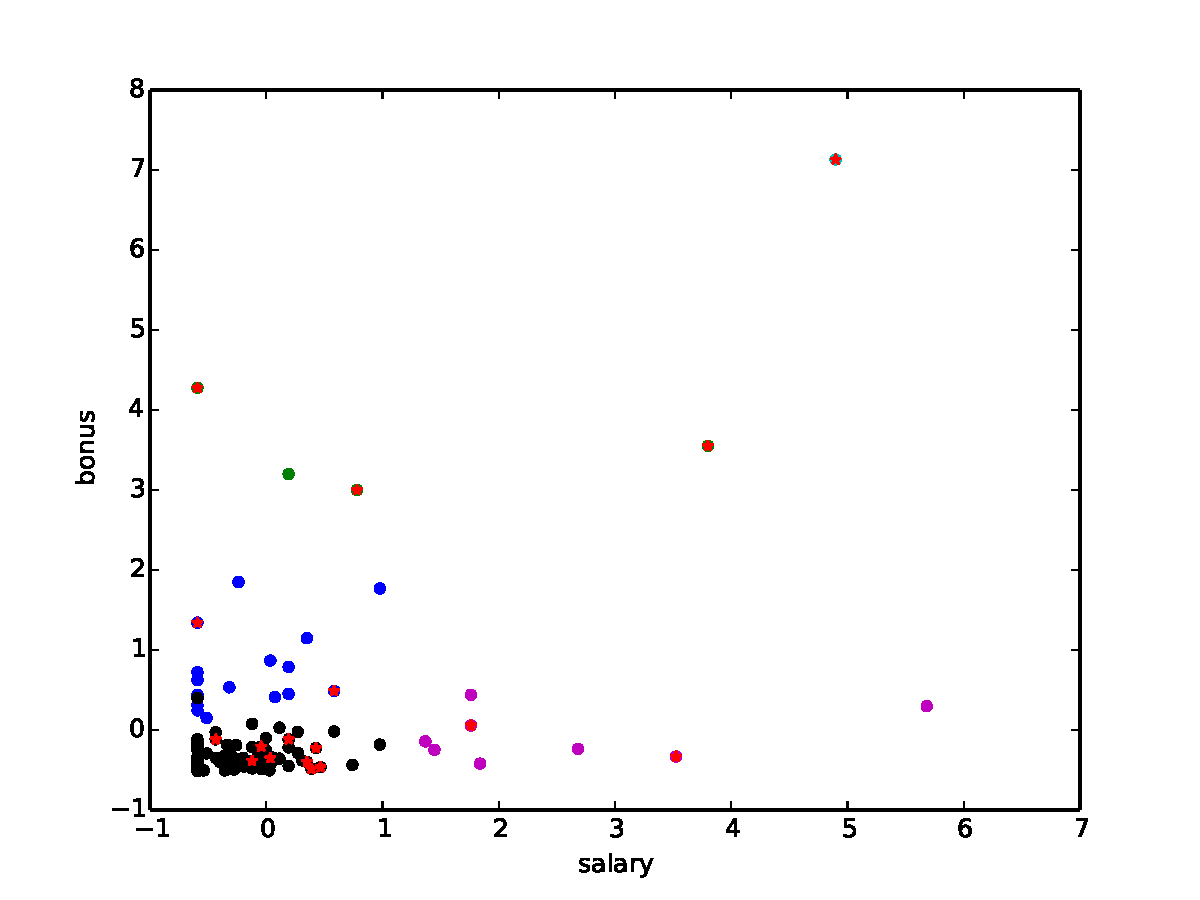
\includegraphics[width=4.3in]{clusters_after_scaling.pdf}
\caption{The results of k-means clustering, with $n_cluster = 5$. Real POIs are marked with stars.}
\end{figure}

Actually it was because of these lines of codes:
\begin{lstlisting}[language=Python,keywordstyle=\color{blue!70},commentstyle=\color{red!50!green!50!blue!50},frame=shadowbox, rulesepcolor=\color{red!20!green!20!blue!20}]
        if prediction == 0 and truth == 0:
            true_negatives += 1
        elif prediction == 0 and truth == 1:
            false_negatives += 1
        elif prediction == 1 and truth == 0:
            false_positives += 1
        else:
            true_positives += 1
\end{lstlisting}
When n\_cluster was set to larger than 2, it meant the predictions would have more than two kinds of values, but all of them except 0 and 1 went into the last `else' condition and made the precision incorrectly high. I trained and validated this classifier in the whole dataset, which is acceptable for an unsupervised algorithm, and evaluated correctly. The precision/recall could vary from 0.1 to 0.6, but could never be as high as 0.9. The idea of using n\_cluster $>$ 2 seems ridiculous. However, in principle, it might be justified somehow. There could be different subgroups in POIs, then the clustering might run poorly with two clusters, but becomes better when using more then eventually combines several clusters in to one.
\section{Notes}
The codes for the exploration with different numbers of features in univariate feature selection and the tuning were commented out in the final version. To run them, you can checkout commit\\
3f6ac95eafc2d78c80d09251123be1081e973162 (at GNB branch),\\
c45020117a97af499694bd979cb5c26b4e019ce6 (at master branch, for univariate feature selection)
and \\
e0ed173105851a89cc121aa3aeacbb18f31705cd(at master branch, tuning).


\end{document}

